%\begin{equation}\label{eq. X16}
%	F = PLw 
%\end{equation}

% need to talk about pressure force length and width in the design section. keep high high level, only enough for the reader to understand the thought process behind torque generation

\begin{figure}[t!]
\centering
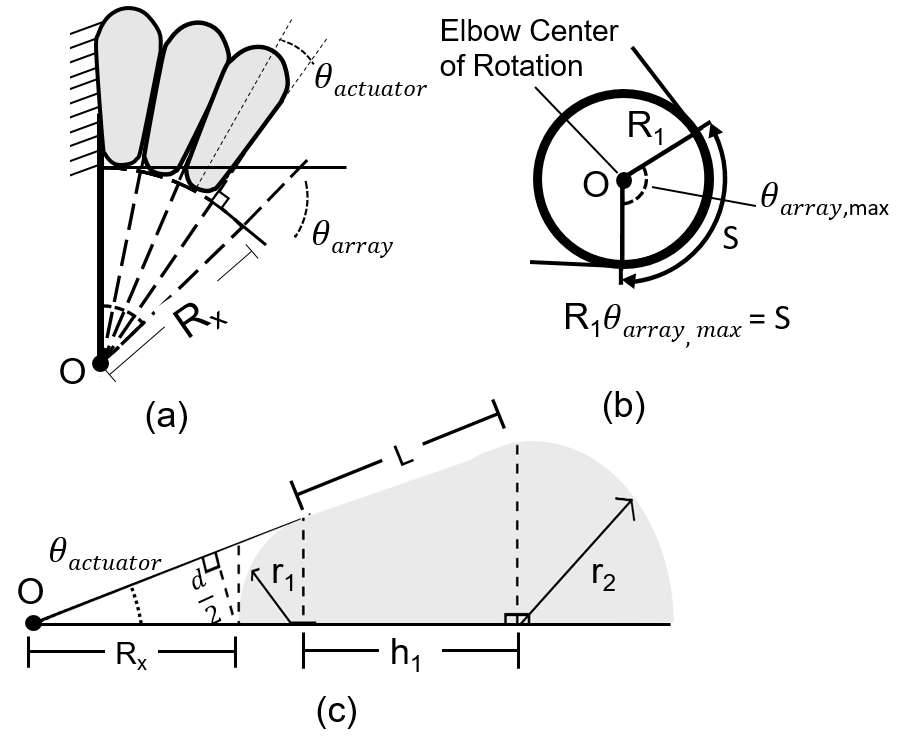
\includegraphics[width=0.35\textwidth]{model3.PNG}
\caption{(a) Arc length model used to determine total actuator length. (b) Simple two bladder arrangement demonstrating $R_x = \infty$. (c) The inextensible layer joining adjacent bladders at the base of the device, with length, $d$, is assumed to be curved as it cumulatively arches to reach the elbow bending angle, $\theta_0$ }
\label{fig:hotness}
\end{figure}
%\textcolor{red}{S=R1theta0 and theta1 is centerline to interacting edge }

Modeling the torque output of the actuator array follows the same geometric principles outlined in Section IVA. However, line contact across two actuators is replaced with the interacting area to account for shape deformation. Additionally, the array of actuators is removed from free-space bending and constrained to the elbow.  When pressurized, the resultant shape of the actuators is shown in Fig \ref{fig:hotness}a.  

 Upon closer inspection of the individual actuator, it is observed that the shape resembles that of a right triangle with a quarter circle attached to the end (Fig. {hotness}c).  Using this shape as the foundation for the following torque model, we can utilize fundamental trigonometric and geometric equations to define the required dimensions needed to calculate the reaction force of the actuators described in Eq. \ref{torq}. Using the tangent relationship, the minor radius is determined to be 
 

\begin{equation}\label{r1}
	r_1(\theta_1)  = \frac{dR_x}{2R_xcos(\theta_1)}
\end{equation}
 where R1, is the radius of the elbow joint. Utilizing the same tangent relationship with the addition of geometrical dimensions and algebraic manipulation, the major radius r2 can be reduced to a second order polynomial with the solution as
 \begin{equation}\label{r2}
	r_2(\theta_1)  = -b + \sqrt{\frac{b^2-4ac}{2a}}
\end{equation}

where a, b, and c are the coeficients of the polynomial. Since the geometry about the centerline of the actuators is assumed to be equal, a half  perimeter of the circle is used to compute the length of interaction
 \begin{equation}\label{L}
	L(\theta_1)  = \frac{\pi}{2}(r_1+r_2) -\pi R
\end{equation}

Using Eq r1, r2, and L as is, is unrepresentative of what the actual behavior of the 


The total length of the actuator array is represented by
\begin{equation}\label{S}
	S = R_1\theta_{max}
\end{equation} 
where  $S$ is the arc length, $R_1$ is the radius of a spherical elbow joint, and  $\theta_{max}$ is the maximum bending angle of the elbow (Fig. \ref{fig:hotness}b). The reason why S is defined as such, is because when it is constrained to the elbow joint thats bent at the maximum angle, additonal length of S does not provide any additional "stuff"

Since torque is dependent on the moment arm $L_F$ (as seen in Eq. \ref{torq}), any additional length and/or number of actuators past the retainer, has no effect on the torque output.

The arclength of $S$ is assumed to have the same terminating angle as the elbow.  This relationship is shown by

\begin{equation}\label{Rx2}
	R_x(\theta) = R_1\frac{\theta_{max}}{\theta}
\end{equation}
where $R_x$  is  the radius of curvature at the current angle $\theta$.  At $\theta_{max}$, $R_x$ is equal to $R_1$, therefore the same relationship is used to define the curvature radius  as bending angle varies through the elbow's flexion and extension. The equation demonstrates that $R_x$ will range from $R_1$ to ${\infty}$, which is portrayed in Fig. \ref{fig:Model1}.\textcolor{red}{Come Back}
% TMI - Figure \textcolor{red}{BOOM B} demonstrates that the range of $R_x$ must vary from ${\infty}$ to $R_{1}$ as the elbow bends from full extension through its full range of motion as it has an inverse dependence on $\theta_0$.   

Since the actuators are symmetrical about the radial centerline, the cross-section, shown in Fig. \ref{fig:hotness}(c), is used to extract remaining dimensions needed to calculate their reaction forces, i.e. $L$ and $w$.

%\textcolor{red}{replace L1 with h1 spanning the entire length of the actuator (at the bottom)}. That is not theta1 }


\begin{equation}\label{L}
	L(\theta_1)  = \frac{\pi}{2}(r_1+r_2) -\pi R
\end{equation}

\begin{equation}\label{r1}
	r_1(\theta_1)  = \frac{dR_x}{2R_xcos(\theta_1)}
\end{equation}
 
 \begin{equation}\label{r2}
	r_2(\theta_1)  = -b + \sqrt{\frac{b^2-4ac}{2a}}
\end{equation}

Equation \ref{L} is the perimeter length of a semi circle and is used to define the relationship between $L$ and the inner and outer radius, $r_1$ and $r_2$, respectively. The inner radius, $r_1$, is found through its tangent relationship with respect to $d$, the equidistant length between the actuators, and $R_x$ (Eq. \ref{r1}); $r_2$ is found utilizing the same trigonometric function in addition to simple geometrical substitutions that lead to a second order polynomial (Eg. \ref{r2}). Substitution of Eg. \ref{r1} and Eg. \ref{r2} into Eg. \ref{L} results in one of the two area of interaction parameters. 
%Equations \textcolor{red}{BOOM} and \textcolor{red}{BOOM} is input into Eq. \textcolor{red}{BOOM BOOM} to find the $L$. 

Although a uniform cross-section of the actuator has sufficiently represented its geometries, to assume a constant width, $w$, as discussed in Section II, would result in an over estimated force model. The rectangular actuators do not retain the same longitudinal cross-section dimensions when pressurized, witnessed in previous work and studies conducted on inflatable actuators (\cite{Natividad2017}). Therefore, an adjusted effective width, $w_1$, is required to better represent the behavior of the actuators. 

\begin{equation}\label{w1}
	w_1(\theta_1)  = w_0-2R(1-\frac{h_1(\theta_1)-2R}{h_0-2R})
\end{equation}


It is assumed that the actuator ends reduce in section width to form a cylinder shape when allowed to expand fully in free-space. Therefore, a correlation is needed to be drawn between it and another dimension dependent on $\theta_1$. Variable height, $h_1$, is chosen as its value is assumed to vary proportionally to $w_1$. At a maximum, $h_1$ =  $h$; at a minimum, $h_1$ = $2R$. Depending on the ratio of heights, the effective width will be reduced proportionally by the product of the ratio and $2R$. 

Utilizing Eq. (\ref{L}) and (\ref{w1}) to measure the effective area of interaction, a bending angle of 90$^{\circ}$ degrees is used as the variable input into the equation 

\begin{equation}\label{torque}
	T(\theta_1) = PLL_Fw_1
\end{equation}

to calculate the theoretical torque generated by the exosuit, where $P$ is the pressure input parameter. 


 %Therefore, an approximation is made on the effective width, $w_1$, in contact. It was assumed that reduction from initial width, $w_0$, is dependent on the ratio of the inflated actuator's height, $h_1$ to initial height, $h_0$ (eq. 8). 

%Once $\textit{L}$ was determined, the effective force was calculated, and therefore, the torque it would generate about the elbow joint. Since pressure, $\textit{P}$ is equal at every point within the inside of the actuator, force, $\textit{F}$ is also distributed evenly across the interacting area ($L\cdot w_{1}$) and is represented as a point load applied at $L_f$, the distance from the axis of rotation to the center of $L$.

%Various inputs, i.e. actuator heights, quantity of actuators and a 90 degree bending angle, were used to assess their resultant torque values (Fig. 8). The three main considerations for inputs were based on design constraints in which the remaining parameters are derived from them. Pressure input, $P$,  was set to a safe limit determined through preliminary testing of individual actuators, with reliable resistance to bursting up to 275kPa. Torque and pressure have linear dependencies as shown in Eq.  9 and 10, therefore only one set pressure was modeled for. 